\documentclass[12pt,oneside,a4paper]{article} % for submission
%\documentclass[12pt,oneside,a4paper]{article} % for sharing

\usepackage{amsmath}
\usepackage{caption}
\usepackage{graphicx}
\usepackage{array}
\usepackage{longtable}
\usepackage{booktabs}
\usepackage[margin=1in]{geometry}

% columnt-types to arrange longtable
\newcolumntype{C}[1]{>{\centering\let\newline\\\arraybackslash\hspace{0pt}}m{#1}}
\newcolumntype{L}[1]{>{\raggedright\let\newline\\\arraybackslash\hspace{0pt}}m{#1}}


\begin{document}
\setcounter{table}{1}

\begin{longtable}{m{0.15\textwidth}L{0.5\textwidth}C{0.2\textwidth}}
  \caption{All dyadic juxtapositions of the six measures of demographic time.}
  \label{tab:dyads}\\
 
  \toprule
  \multicolumn{3}{m{0.9\textwidth}}{\footnotesize \emph{Note:} The temporal
  planes are named after the two given time scales. The derived scale is appended in parentheses. Contrary to mathematical convention we name the ordinate scale first and the abscissa scale second. This is to be consistent with the established APC and ACP terms.} \\
   \midrule
  %%%%%%%%%%%%%%%%%%%%%%%%%%%%%%%%%%%%%%%%%%%%%%%%%%%%%%%%%%%%%%%%%%%%%%%%%%%%%
  \multicolumn{3}{c}{\textsc{Variants of APC}} \\
  \midrule
  %%%% APc
  $$\begin{aligned}
    &\text{AP(C)} \\
    &\text{C = P -- A}
  \end{aligned}$$ &
  The AP(C) temporal plane constitutes the classical Lexis diagram. &
  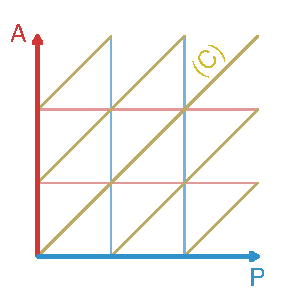
\includegraphics[scale=.5]{Tab201.pdf}
  \\
  %%%% ACp
  $$\begin{aligned}
    &\text{AC(P)} \\
    &\text{P = C + A}
  \end{aligned}$$ &
  The AC(P) temporal plane is equivalent to the Lexis diagram except birth
  cohort is given and period is derived rather than the other way around. &
  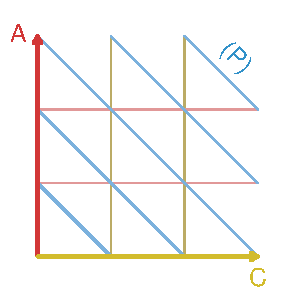
\includegraphics[scale=.5]{Tab202.pdf} 
   \\
  %%%% CPa
  $$\begin{aligned}
    &\text{CP(A)} \\
    &\text{A = P -- C}
  \end{aligned}$$ &
  The CP(A) temporal plane is equivalent to the Lexis diagram except birth
  cohorts are given and age is derived rather than the other way around. &
  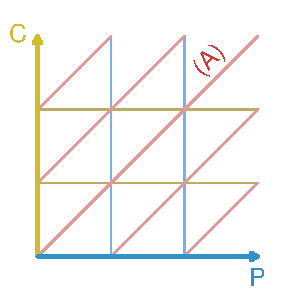
\includegraphics[scale=.5]{Tab203.pdf}  
  \\
  \midrule
  %%%%%%%%%%%%%%%%%%%%%%%%%%%%%%%%%%%%%%%%%%%%%%%%%%%%%%%%%%%%%%%%%%%%%%%%%%%%%
  \multicolumn{3}{c}{\textsc{Variants of TPD}} \\
  \midrule
  %%%% TPd
  $$\begin{aligned}
    &\text{TP(D)} \\
    &\text{D = P + T}
  \end{aligned}$$ &
  Helen had 30 years of life left (T) in 1971 (P) and therefore belonged to the 2001 death cohort (D) &
  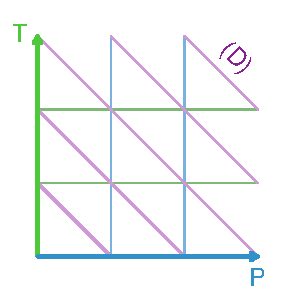
\includegraphics[scale=.5]{Tab204.pdf}  
   \\
  %%%% PDt
  $$\begin{aligned}
    &\text{PD(T)} \\
    &\text{T = D -- P}
  \end{aligned}$$ &
  Mindel died in 1973 (D). In 1953 (P) she had 20 years left to live (T). &
  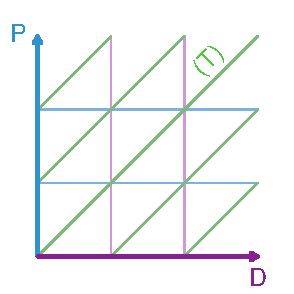
\includegraphics[scale=.5]{Tab205.pdf} 
   \\
  %%%% TDp
  $$\begin{aligned}
    &\text{TD(P)} \\
    &\text{P = D -- T}
  \end{aligned}$$ &
  Irene died in 1974 (D). When she had 30 remaining years of life (T) the year must have been 1944 (P). &
  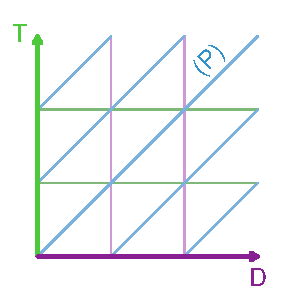
\includegraphics[scale=.5]{Tab206.pdf}   
  \\
  \midrule
  %%%%%%%%%%%%%%%%%%%%%%%%%%%%%%%%%%%%%%%%%%%%%%%%%%%%%%%%%%%%%%%%%%%%%%%%%%%%%
  \multicolumn{3}{c}{\textsc{Variants of TAL}} \\
  \midrule
  %%%% TAl
  $$\begin{aligned}
    &\text{TA(L)} \\
    &\text{L = T + A}
  \end{aligned}$$ &
  The time already lived and the time still left sum up to the total lifespan. &
  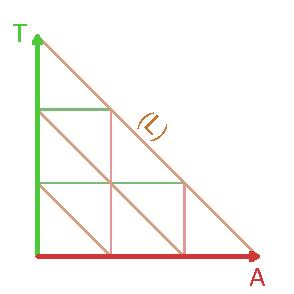
\includegraphics[scale=.5]{Tab207.pdf}   
  \\
  %%%% TLa
  $$\begin{aligned}
    &\text{TL(A)} \\
    &\text{A = L -- T}
  \end{aligned}$$ &
  Helen lived to the age of 86 (L). When she had 20 years left (T) she must have been 66 (A). &
  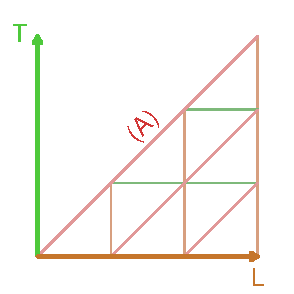
\includegraphics[scale=.5]{Tab208.pdf}   
 \\
  %%%% ALt
  $$\begin{aligned}
    &\text{AL(T)} \\
    &\text{T = A -- L}
  \end{aligned}$$ &
  Tim is 34 years old (A) and will live to the age of 96 (L), leaving him 62 years (T) to settle affairs. &
  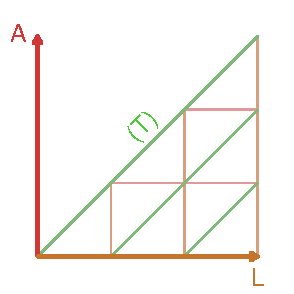
\includegraphics[scale=.5]{Tab209.pdf} 
  \\
  \midrule
  %%%%%%%%%%%%%%%%%%%%%%%%%%%%%%%%%%%%%%%%%%%%%%%%%%%%%%%%%%%%%%%%%%%%%%%%%%%%%
  \multicolumn{3}{c}{\textsc{Variants of LCD}} \\
  \midrule
  %%%% LCd
  $$\begin{aligned}
    &\text{LC(D)} \\
    &\text{D = C + L}
  \end{aligned}$$ &
  \`{A}ngels was born in 1940 (C) and she lived to be 64 (L), implying an
  untimely death in 2004 (D) &
  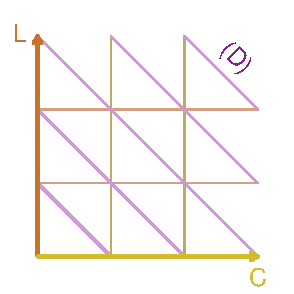
\includegraphics[scale=.5]{Tab210.pdf}   
  \\
  %%%% CDl
  $$\begin{aligned}
    &\text{CD(L)} \\
    &\text{L = D -- C}
  \end{aligned}$$ &
  Pascal was born in 1893 (C) and died in 1964 (D), implying a lifespan of 71 (L), or so. &
  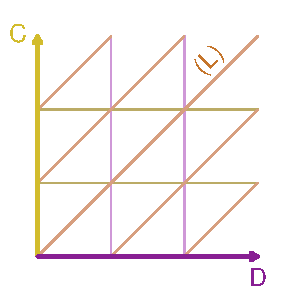
\includegraphics[scale=.5]{Tab211.pdf} 
  \\
  %%%% LDc
  $$\begin{aligned}
    &\text{LD(C)} \\
    &\text{C = D -- L}
  \end{aligned}$$ &
  Margaret died in Dec., 1995 (D) with a completed lifespan of 96 (L), putting her birth year in 1900 (C). &
  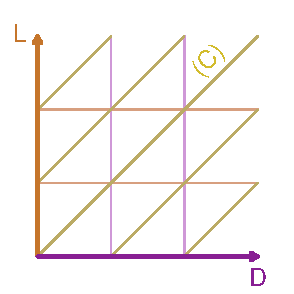
\includegraphics[scale=.5]{Tab212.pdf}  
  \\
  \midrule
  %%%%%%%%%%%%%%%%%%%%%%%%%%%%%%%%%%%%%%%%%%%%%%%%%%%%%%%%%%%%%%%%%%%%%%%%%%%%%
  \multicolumn{3}{c}{\textsc{The Uninformative Dyads}} \\
  \midrule
  %%%% LP
  LP(-) &
  The LP plane is \emph{non-informative}. No additional measures can be derived knowing just lifespan and period. &
  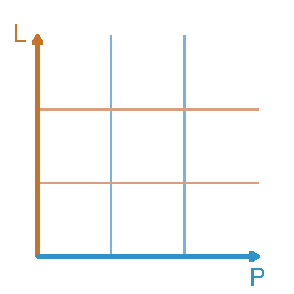
\includegraphics[scale=.5]{Tab213.pdf} 
  \\
 %%%% CT
  CT(-) &
  The CT plane is \emph{non-informative}. No additional measures can be derived
  knowing just birth cohort and thanatological age. &
  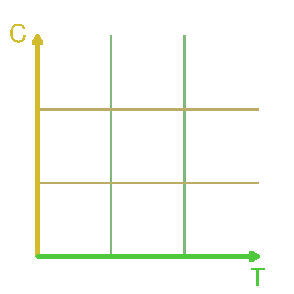
\includegraphics[scale=.5]{Tab214.pdf} \\
  %%%% AD
  AD(-) &
  The AD plane is \emph{non-informative}. No additional measures can be derived
  knowing just death cohort and age. &
  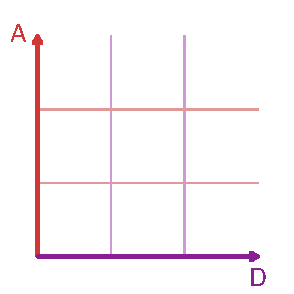
\includegraphics[scale=.5]{Tab215.pdf} 
\\
  \bottomrule
\end{longtable}

\end{document}